\documentclass{proc}

\usepackage{hyperref}
\usepackage{listings}
\usepackage{graphicx}
\usepackage{float}
\usepackage{amssymb}
\usepackage{amsmath}


\newcommand{\noun}[1]{\textsc{#1}}

\begin{document}

\title{Concepts tool - Manual}
\author{Jonathan Beaumont\\
\texttt{j.r.beaumont@ncl.ac.uk}\\
\emph{School of Electrical and Electronic Engineering, Newcastle University,UK}\\\\
Last updated \today}

\maketitle

\tableofcontents

\onecolumn

\section{Introduction}

\emph{Concepts} are a formal method of specifying asynchronous circuits. With concepts, one can describe behaviours of a circuit and its environment at various levels, with the aim of
defining the behaviours in terms of gates, protocols or simple signal interactions. Using this method, one can split a design into scenarios, based on operational modes, individual functions, or 
any other method a user decides. These can be specified separately, using concepts, and then combined to provide a full system specification. Through this, reuse is promoted,
 allowing concepts to be reused between scenarios and even entire designs. More information on the theory of concepts can be found in~\cite{2016_beaumont_concepts}, the latest version 
of which can be found \href{https://github.com/tuura/concepts-article/releases}{here}.

In this document, we will discuss the associated tool for concepts. This open source tool is written in \emph{Haskell}, and contains both the library for concepts, 
including abstract concepts and circuit concepts built upon the abstract, and a tool for translating concepts into \emph{Signal Transition Graphs}~(STGs)~\cite{Chu_1987_phd}
\cite{Rosenblum_1985_tpn}. These are commonly used for the specification, verification and synthesis of asynchronous control circuits in the academic community, and 
they are supported by multiple EDA tools, such as \noun{Petrify}~\cite{Cortadella}, \noun{Mpsat}~\cite{khomenko2004detecting}, \noun{Versify}~\cite{i1997formal}, 
\noun{Workcraft}~\cite{2007_poliakov_workcraft}\cite{Workcraft_website}, and others.  
The aim of this tool is to design and debug concepts, and then translate them to STGs, where they can be used with these tools. 

The latest version of this tool, and this manual, can be found \href{https://github.com/tuura/concepts}{in the GitHub repo}. Any bugs or issues found with the tool can be reported here. 
This tool is also distributed as a back-end tool for \noun{Workcraft}. This version of the concepts tool will be the latest version that works correctly with \noun{Workcraft}. The latest 
version of \noun{Workcraft}, which also features tools  such as \noun{Petrify} and \noun{Mpsat}, can be downloaded from \url{http://workcraft.org/}. 

\section{Installation}

The concepts tool, as well as \noun{Workcraft} are available for \emph{Windows}, \emph{Linux} and \emph{Mac OS X}. The installation instructions for all of these operating systems are 
the same. We will be referring to directories using the \\forward-slash character ('/') as a separator, however for \emph{Windows}, replace this with a back-slash character 
('\textbackslash').

If choosing to use the concepts tool on its own, this must be 
downloaded from the \href{https://github.com/tuura/concepts}{GitHub repo}. If you choose to use this tool as part of \noun{Workcraft}, download this from the 
\href{http://workcraft.org/}{\noun{Workcraft} website}. Once downloaded, extract the contents of the folder, and move them to a directory you wish to run them from. 

\subsection{Concepts tool requirements\label{sub:Concepts_requirements}}

The concepts tool is written in \emph{Haskell}, and uses \emph{Stack} to install the necessary compiler and dependencies. If necessary, please download stack for your operating 
system, available from \url{https://haskell.org/downloads#stack}, and follow the instructions to install this.

\subsection{Workcraft requirements}

\noun{Workcraft} is written in Java, and the latest version of the \emph{Java Runtime Environment}~(JRE) needs to be installed to run.  This can be downloaded from 
\url{http://java.com/en/download/}. If needed, download the JRE installer, and follow the instructions to install this.

While the concepts tool is distributed with \noun{Workcraft}, it still needs to be built by \emph{stack} in order for it to be run. 
See Section~\ref{sub:Concepts_requirements} for requirements for the concepts tool.

\newpage
\subsection{Installing the tool}

Once either the concepts tool or \noun{Workcraft} has been extracted and moved to the desired directory, using command line, navigate to the concepts tool directory, or if using 
\noun{Workcraft}, navigate to the \noun{Workcraft} directory, and then navigate to the concepts tool directory, found in \texttt{tools/concepts} (for \emph{OS X}, the 
\noun{Workcraft} directory is located within the \texttt{Workcraft.app} contents folder. The concepts tool will be found at \texttt{Contents/Resources/tools/concepts}.

Now, the process of installing the tool is the same, regardless of how you aim to use the concepts tool. First of all, let's setup stack. To do this, run: 

\begin{lstlisting}[language=bash]
  $ stack setup
\end{lstlisting}

This will prepare stack to install the concepts tool. Now, to build and install the concepts tool, simply run:

\begin{lstlisting}[language=bash]
  $ stack build
\end{lstlisting}

If this process completes successfully, the tool will now be installed and ready to be used.

\section{Using the tool from command line}

With the tool installed, we can now start to use it to translate concepts to STGs. We will begin by discussing how it is used from command line. Usage as a back-end tool in 
\noun{Workcraft} is discussed in Section~\ref{sec:workcraft_usage}.

The standard command for the tool is as follows:

\begin{lstlisting}[language=bash]
  $ stack runghc <path-to-translate> <path-to-concepts-file> 
                                           [--stack-yaml <path-to-stack-file>]
\end{lstlisting}

The three parts of this are as follows:
\begin{itemize}
  \item \texttt{stack} - This will ensure that the dependencies and compiler are installed when running.
  \item \texttt{runghc} - This runs the translation function.
  \item \texttt{<path-to-translate>} - This is file path pointing to the translate code file, which performs the necessary operations to translate concepts to STGs.
  \item \texttt{<path-to-concepts-file>} - This is the path pointing to the file containing the concepts to be translated.
  \item \texttt{[--stack-yaml <path-to-stack-file>]} - This is optional. If running the tool from outside of the directory, the path to the stack file needs to be given.
\end{itemize}

When running the concepts tool from command line, as long as the paths to the translate code, the concepts
file and the \texttt{stack.yaml} file are correct, it doesn't matter which directory the tool is run from.  The \texttt{stack.yaml} file is located in the base of the concepts directory.

Now, let's use one of the examples included with the concepts tool to show the usage. These can be found in the \texttt{examples} directory of the concepts tool. 
For this section, we will assume that we are currently in the concepts tool directory. The example we will use is the file titled "\texttt{Celement\_with\_env\_1.hs}". 
This has the ".hs" file extension, as it is in fact a file using Haskell code, and all files containing concepts should feature this file extension. 
To translate this concepts file to an STG, the following command must be run:

\begin{lstlisting}[language=bash]
  $ stack runghc translate/Main.hs examples/Celement_with_env_1.hs
\end{lstlisting}

When the translation is complete, the tool will output the following:

\begin{lstlisting}[language=bash]
  .model out
  .inputs A B
  .outputs C
  .internals
  .graph
  A0 A+
  A+ A1
  A1 A-
  A- A0
  B0 B+
  B+ B1
  B1 B-
  B- B0
  C0 C+
  C+ C1
  C1 C-
  C- C0
  A1 C+
  C+ A1
  B1 C+
  C+ B1
  C1 A-
  A- C1
  C1 B-
  B- C1
  A0 C-
  C- A0
  B0 C-
  C- B0
  C0 A+
  A+ C0
  C0 B+
  B+ C0
  .marking {A0 B0 C0}
  .end
\end{lstlisting}

This output is the STG representation in \emph{.g} format. \emph{.g} files are a standard type used as input to tools, such as \noun{Petrify}, \noun{Mpsat}, and \noun{Workcraft}. 
Therefore, this output can by copy-and-pasted into a file, and saved with the file etension \emph{.g}, and then used as input to these tools. 

The concepts tool can be used in a similar way, ensuring that the file paths to the translate code file, and the concepts input file, are correct. Section~\ref{sec:concepts_layout} contains 
information on how to layout a concepts file, to avoid as many errors as possible. 

Any errors that occur during the translation process will produce errors referring to the problematic lines of signals of the concepts that are problematic. 

\section{Using the tool from \noun{Workcraft} \label{sec:workcraft_usage}}

This section will discuss how to use the concepts tool from within \noun{Workcraft}. There are many other features of \noun{Workcraft}, both as part of the STG plug in, some of which I
 will discuss in the context of concepts here, and as part of other modelling formalisms. More information on these can be found at \url{http://workcraft.org/}.
 
\subsection{Translating and authoring concepts}

First of all, \noun{Workcraft} must be started. This can be done by running the start up script, located in the \noun{Workcraft} directory in \emph{Windows} and \emph{Linux}. In 
\emph{Windows}, this script is named ``\texttt{workcraft.bat}". In \emph{Linux}, it is simply "\texttt{workcraft}". In \emph{OS X}, \noun{Workcraft} can be started instead by double 
clicking the \noun{Workcraft} icon, which is the app container for the necessary files. 

When workcraft starts, you will be greeted by blank screen, as seen in Figure~\ref{fig:blank_workcraft_screen}.

\begin{figure}[H]
\begin{centering}
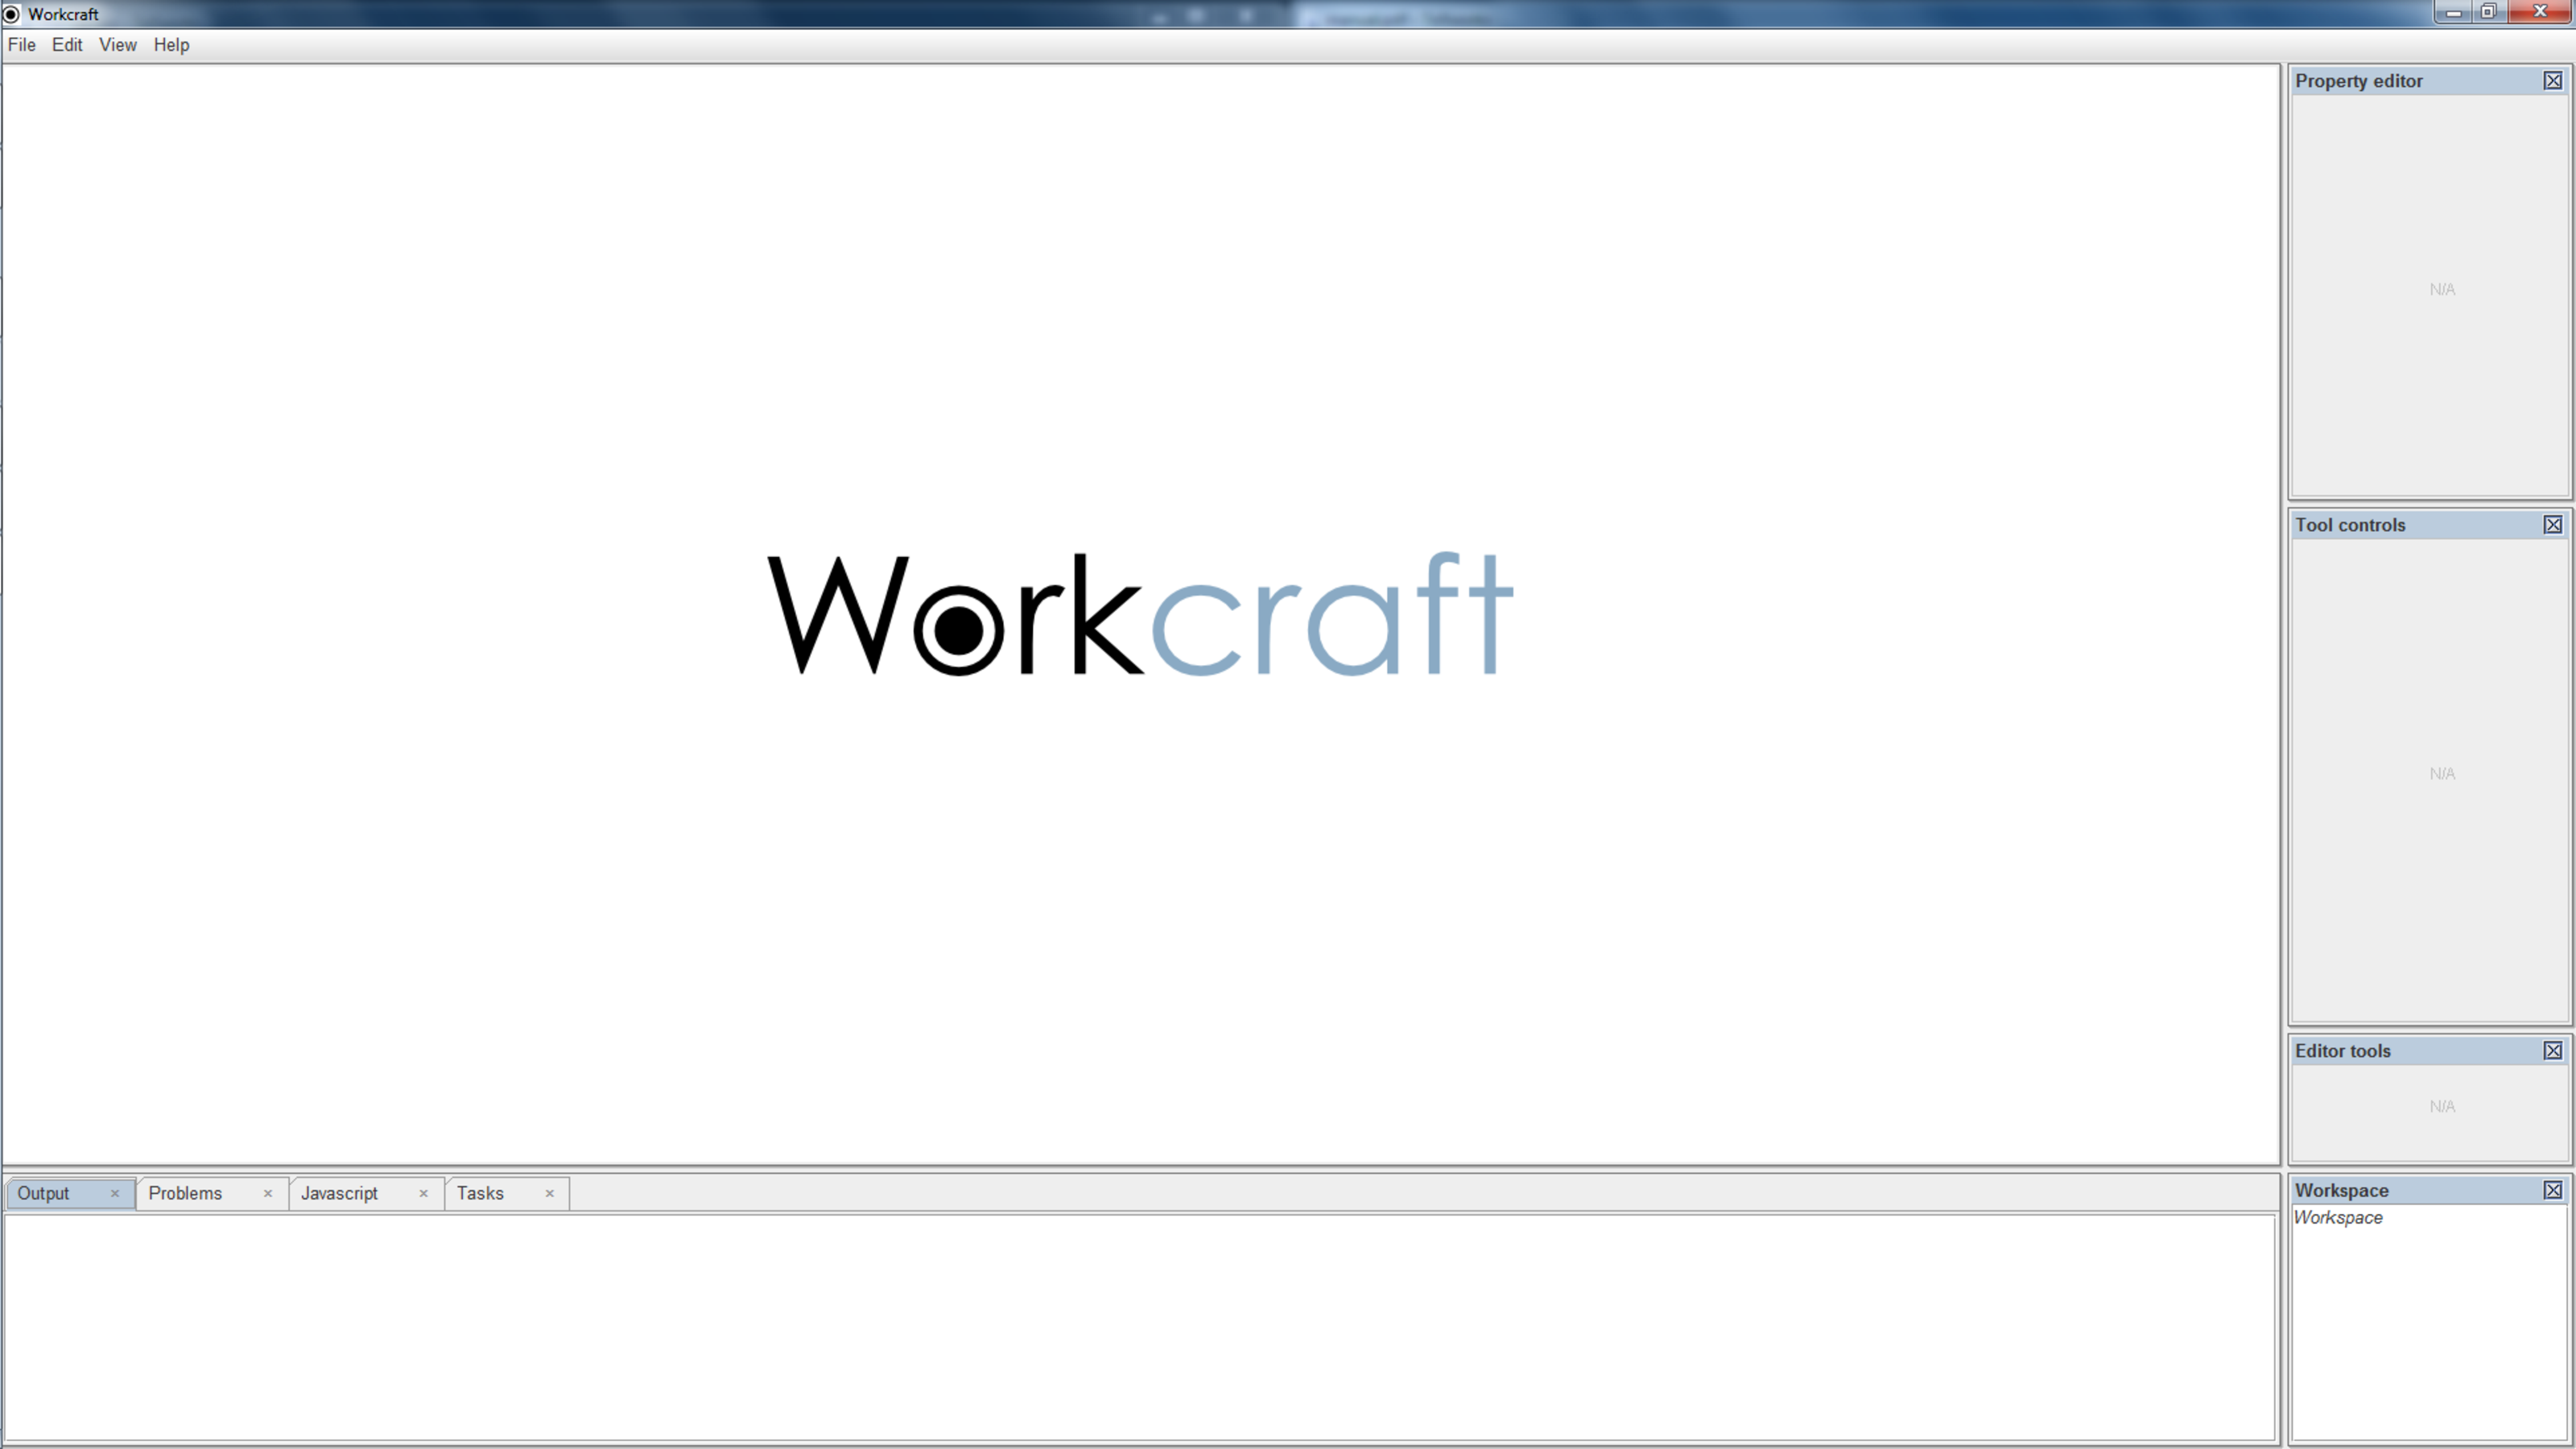
\includegraphics[scale=0.2]{images/blank_workcraft_screenshot}
\par\end{centering}

\begin{centering}
\protect\caption{\label{fig:blank_workcraft_screen}Workcraft immediately after starting.}

\par\end{centering}

\end{figure}

Now, we need to open a new work, specifically a new STG work. Open the "New work" dialog using the menu bar, \texttt{File -> Create work...}, or by pressing \texttt{Ctrl-N} 
(\texttt{CMD-N} on \emph{OS X}). This will bring up a menu as seen in Figure~\ref{fig:new_work_screen}.

\begin{figure}[H]
\begin{centering}
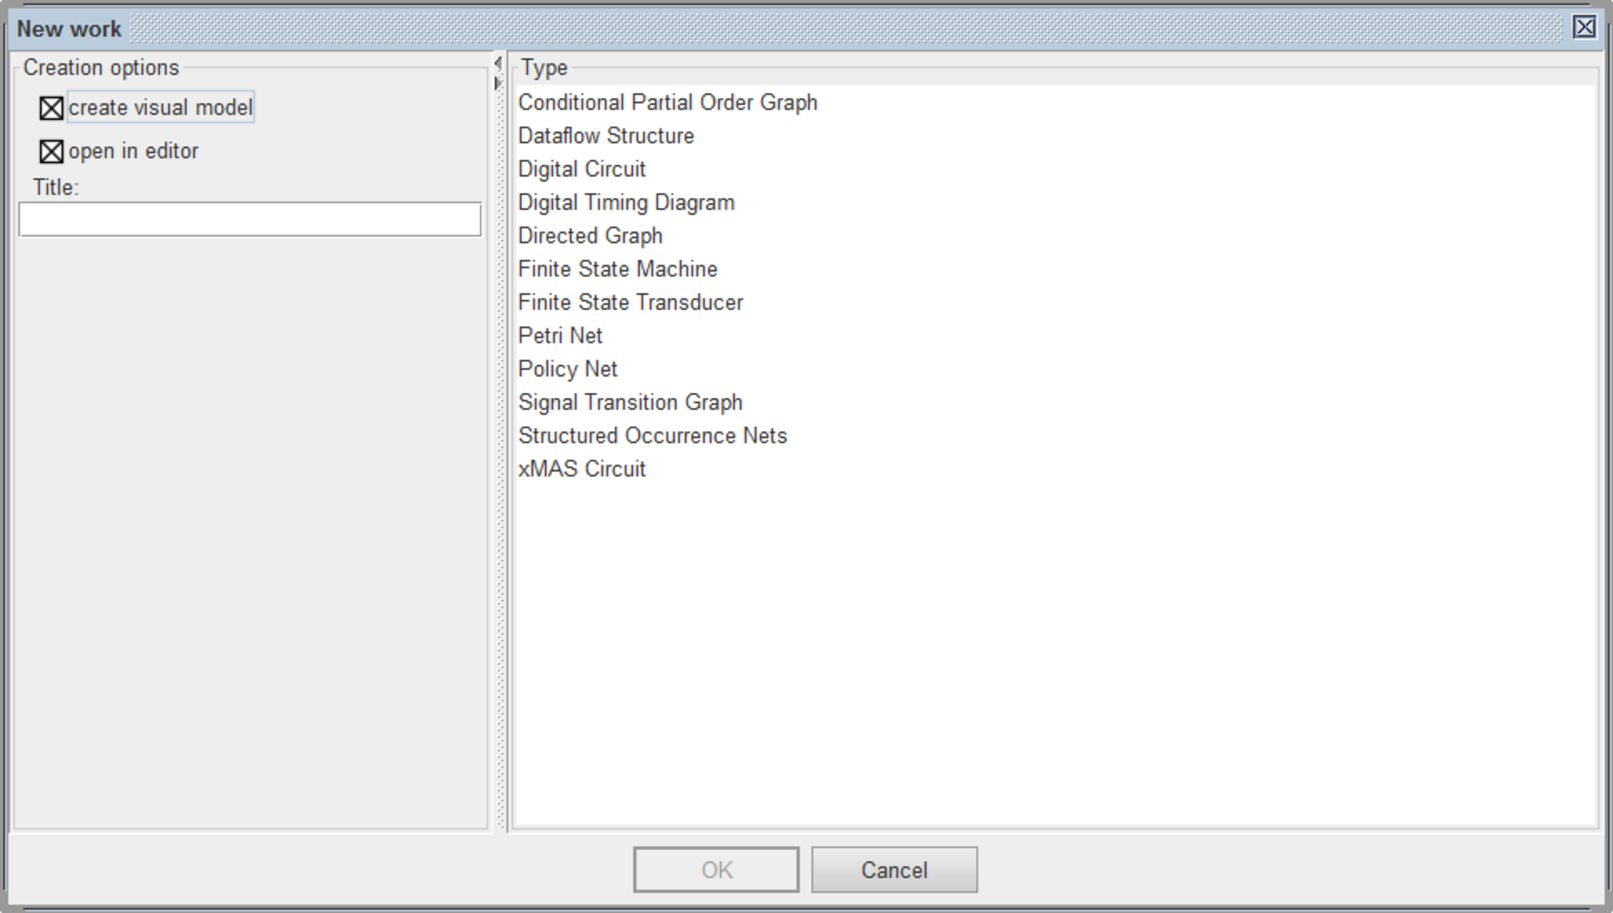
\includegraphics[scale=0.4]{images/new_work_screenshot}
\par\end{centering}

\begin{centering}
\protect\caption{\label{fig:new_work_screen}The create work window.}

\par\end{centering}

\end{figure}

In this window, select ``\emph{Signal Transition Graph}' and cick the ``OK'' button at the bottom of the window. This will the open a blank workspace in which we can create an STG, which 
will look similar to Figure~\ref{fig:blank_stg_work}.

\begin{figure}[H]
\begin{centering}
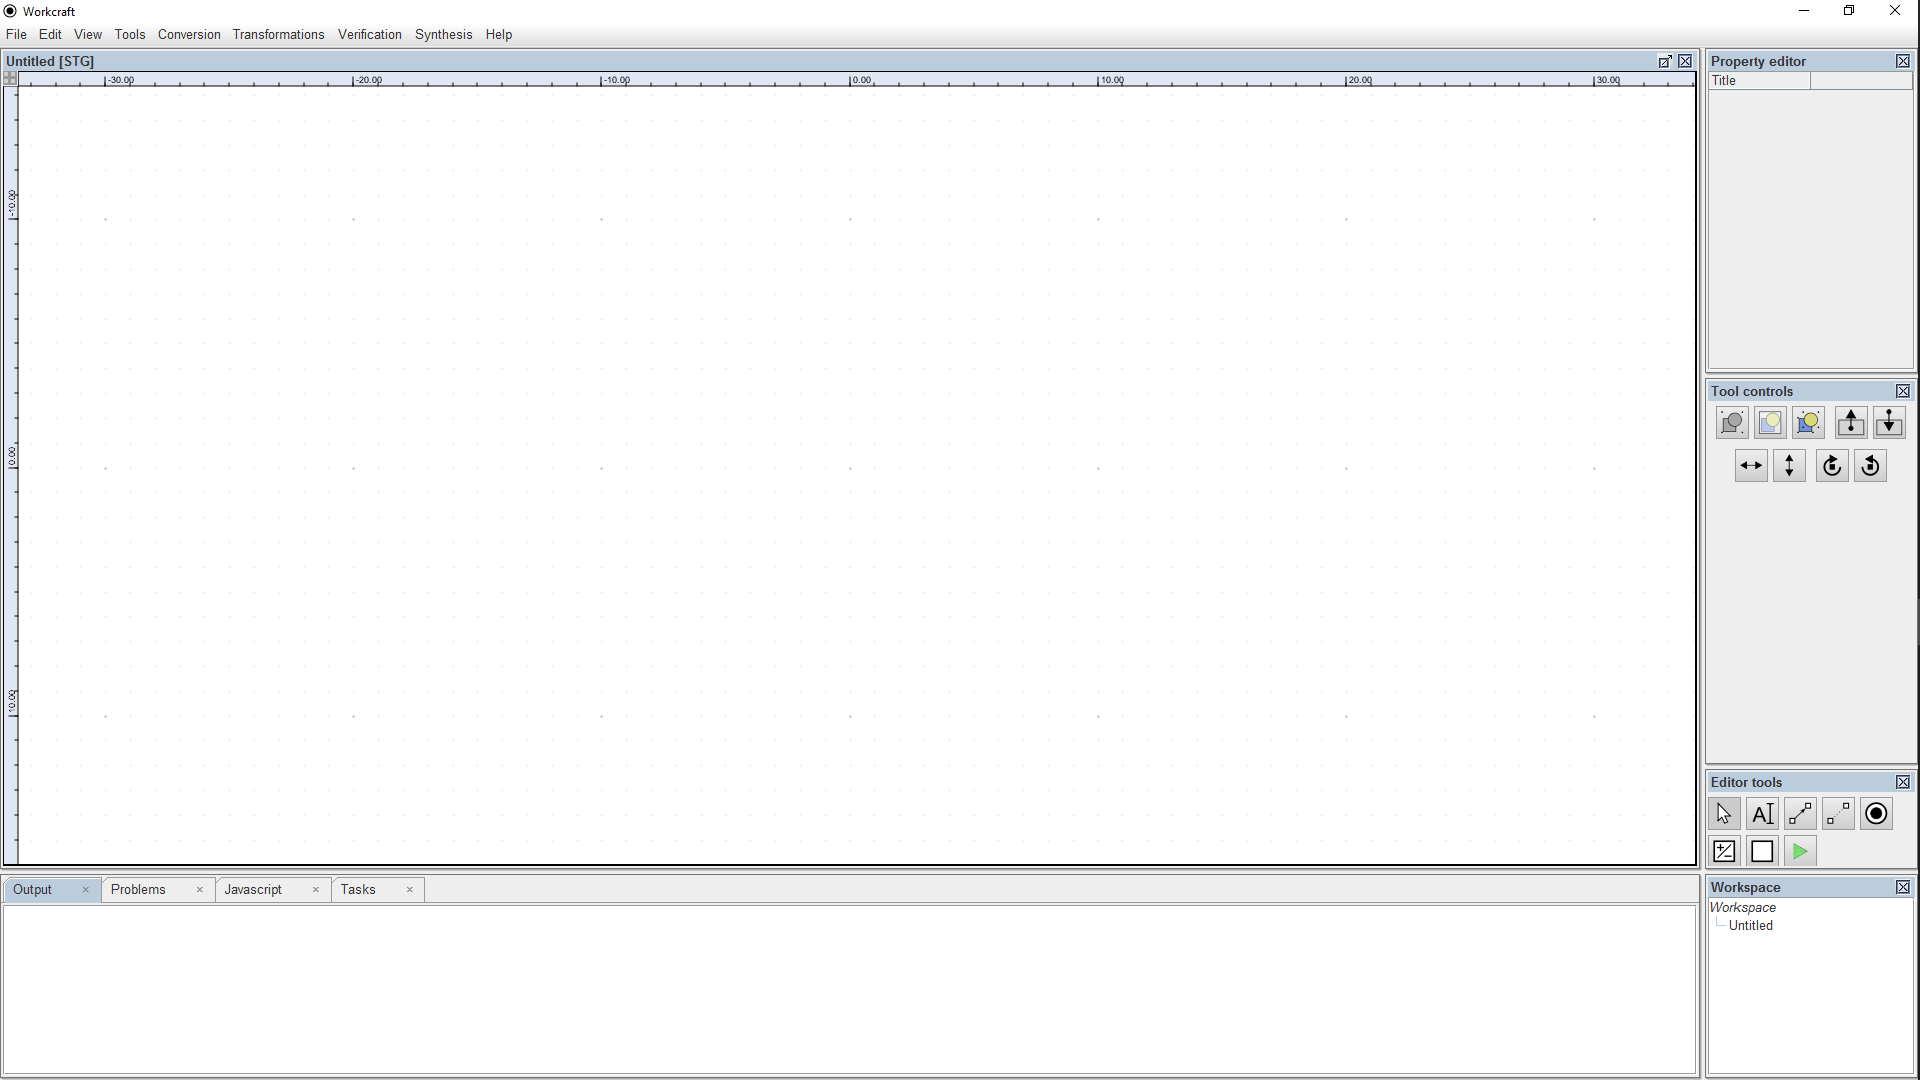
\includegraphics[scale=0.2]{images/new_stg_screenshot}
\par\end{centering}

\begin{centering}
\protect\caption{\label{fig:blank_stg_work}A new STG workspace}

\par\end{centering}

\end{figure}

Now, we can start translating concepts. To do this, first we need to open the concepts dialog.  This is done from the menu bar, by selecting the ``\emph{Conversion}'' menu, and then the 
``\emph{Translate concepts...}'' option. The concepts dialog will look as shown in Figure~\ref{fig:concepts_dialog_screenshot}.

\begin{figure}[H]
\begin{centering}
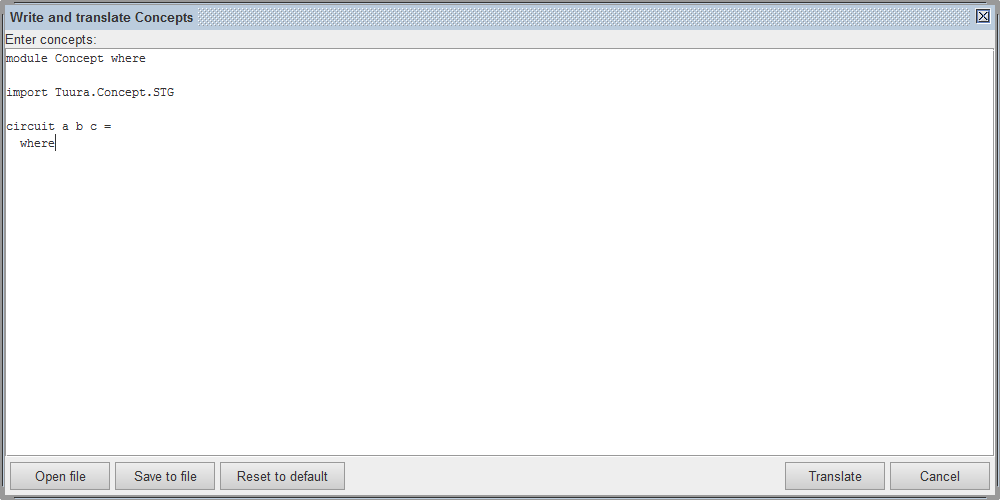
\includegraphics[scale=0.4]{images/concepts_dialog_screenshot}
\par\end{centering}

\begin{centering}
\protect\caption{\label{fig:concepts_dialog_screenshot}The concepts dialog.}

\par\end{centering}

\end{figure}

From within this dialog, one can write their own concepts, from the default template as shown in Figure~\ref{fig:concepts_dialog_screenshot}, or open an existing concepts file, with the  
\emph{.hs} extension. When satisfied with the concepts written, a user can choose to save the file, if not already saved, and then translate these concepts.

\begin{figure}[H]
\begin{centering}
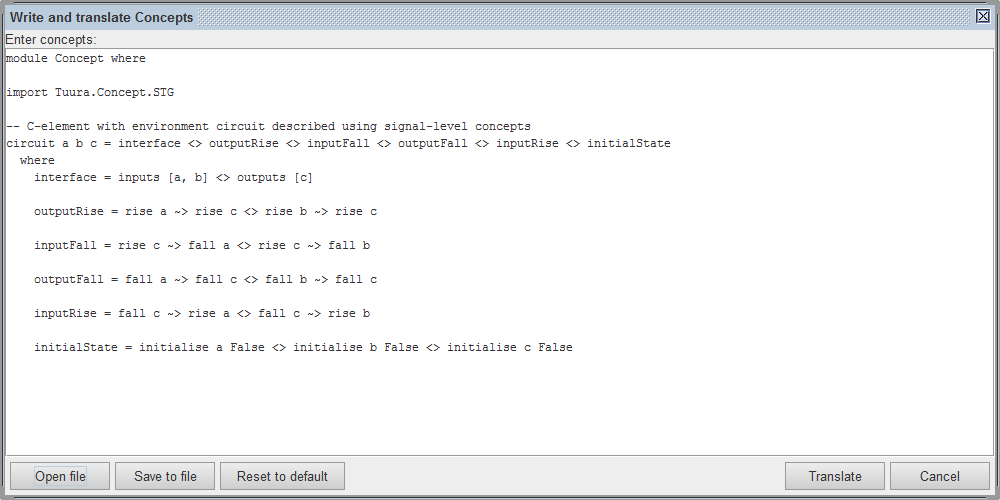
\includegraphics[scale=0.4]{images/concepts_dialog_Celement}
\par\end{centering}

\begin{centering}
\protect\caption{\label{fig:concepts_dialog_Celement}The concepts dialog with a concept file opened.}

\par\end{centering}

\end{figure}

Figure~\ref{fig:concepts_dialog_Celement} is the concepts dialog after we have opened the Celement with environment example, named ``\emph{Celement\_with\_env\_1.hs}'', from the 
concepts tool examples directory. Clicking translate at this point will produce an STG representation of these concepts in the workspace. 

\begin{figure}[H]
\begin{centering}
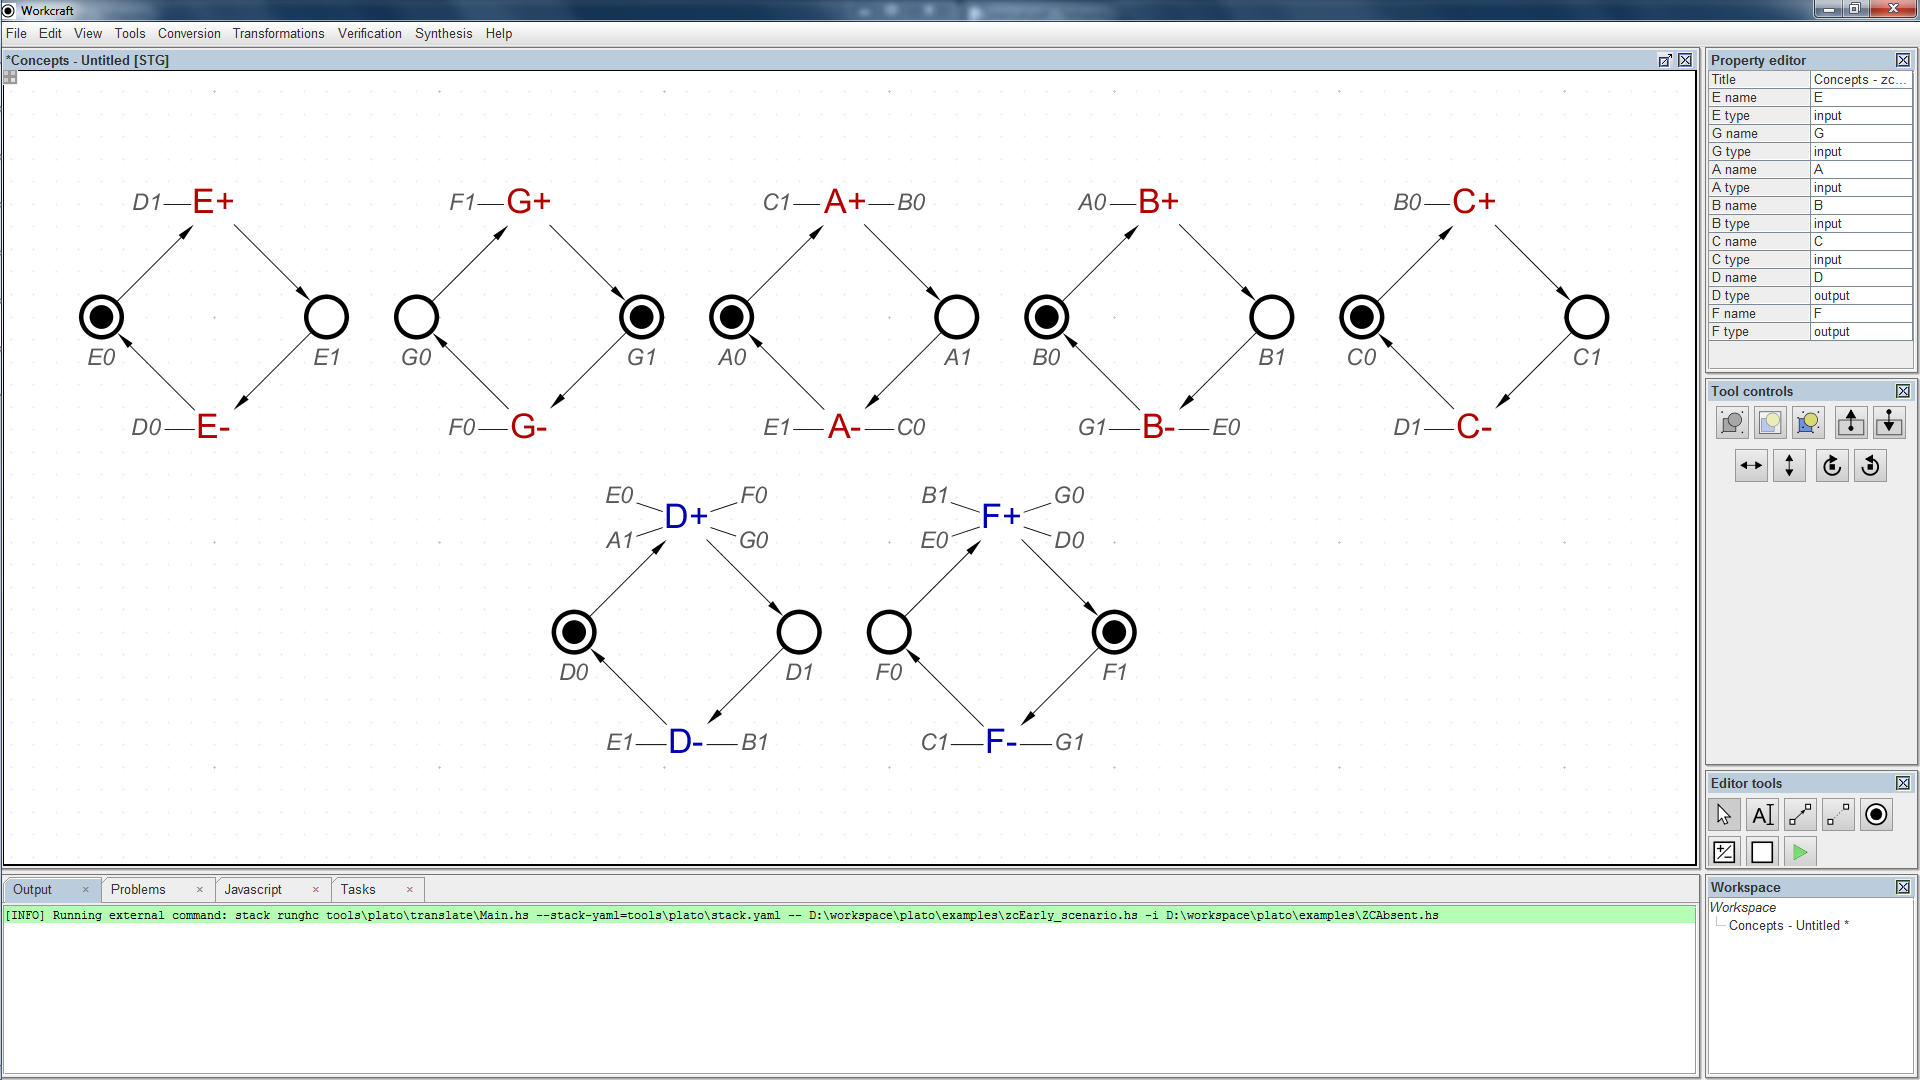
\includegraphics[scale=0.2]{images/concepts_translated}
\par\end{centering}

\begin{centering}
\protect\caption{\label{fig:concepts_translated}The STG produced from translating the concepts.}

\par\end{centering}

\end{figure}

The translated concepts will look similar to Figure~\ref{fig:concepts_translated}

Now, a user can choose to insert more concepts, make changes to this STG, and once they are satisfied with it, can then perform various functions on this STG. One can perform 
transformations, verifications, simulations and synthesis on this STG using the menus within this workspace now. Any further changes to this STG, based on the results of these operations 
can be made to this STG or to the concepts file. 

\subsection{Importing concepts directly}

In \noun{Workcraft} it is also possible to import concepts directly from a file, without having to view the concepts first. 
This can be done from the ``\emph{File}'' menu, by selecting the ``\emph{Import...}'' option. 

\begin{figure}[H]
\begin{centering}
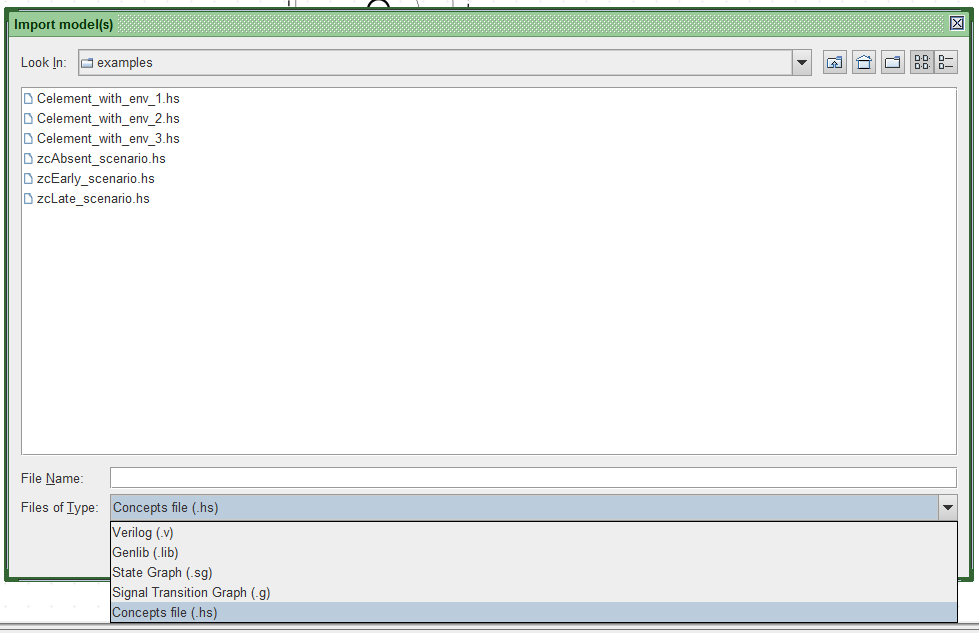
\includegraphics[scale=0.4]{images/import_menu_screenshot}
\par\end{centering}

\begin{centering}
\protect\caption{\label{fig:import_menu_screenshot}The STG produced from translating the concepts.}

\par\end{centering}

\end{figure}

When importing concepts using this menu, ensure to set the ``\emph{Files of Type}'' option to ``\emph{Concepts file (.hs)}'', as shown in Figure~\ref{fig:import_menu_screenshot}

\subsection{Errors}

If any errors are encountered during the translation process, \noun{Workcraft} will produce a helpful error message. 
This usually can tell you with more detail what the issue that is causing the error is, but will ask you to refer to \noun{Workcraft}'s console window for specific line numbers or signals which 
need to be corrected. 
These errors will include whether a signal has not been declared as an input or output,
a signal has not had it's initial state given, or even that the concepts tool has not been installed correctly. 

\section{Writing concepts \label{sec:concepts_layout}}

In this section, we will discuss how to write a concepts file. 
We will use an example and go through it based on lines, explaining what is necessary. For this example we will be using the same 
as example as in previous sections, from the examples included with the concepts repo. This is ``\emph{Celement\_with\_env1.hs}''.

\subsection{Concepts file layout}

\begin{figure}[H]
\begin{centering}

\begin{flushleft}
$\,\mathsf{module}\, Concept \, \mathsf{where}$
\par\end{flushleft}

\begin{flushleft}
$\,\mathsf{import}\, Tuura.Concept.STG$
\par\end{flushleft}

\begin{flushleft}
$\,\mathsf{circuit}\,a \,b \,c=\mathsf{\,interface}\,<> \mathsf{\, outputRise}<>\,\mathsf{inputFall}\,<>\,\mathsf{outputFall}<>\mathsf{\, inputRise}\,<>\,\mathsf{initialState}$

$\,\,\,\mathsf{where}$
\par\end{flushleft}

\begin{flushleft}
$\,\,\,\,\,\,\mathsf{interface}=\mathsf{inputs}\,[a,b]<>\mathsf{outputs}\,[c]$
\par\end{flushleft}

\begin{flushleft}
$\,\,\,\,\,\,\mathsf{outputRise}=\mathsf{rise} \,a\rightsquigarrow \mathsf{rise} \,c\,<>\, \mathsf{rise} \,b\rightsquigarrow \mathsf{rise} \,c$
\par\end{flushleft}

\begin{flushleft}
$\,\,\,\,\,\,\mathsf{inputFall}=\mathsf{rise} \,c\rightsquigarrow \mathsf{fall} \,a \,<>\, \mathsf{rise} \,c \rightsquigarrow \mathsf{fall} \,b$
\par\end{flushleft}

\begin{flushleft}
$\,\,\,\,\,\,\mathsf{outputFall}=\mathsf{fall} \,a \rightsquigarrow \mathsf{fall} \,c \,<>\, \mathsf{fall} \,b \rightsquigarrow \mathsf{fall} \,c$
\par\end{flushleft}

\begin{flushleft}
$\,\,\,\,\,\,\mathsf{inputRise}=\mathsf{fall} \,c \rightsquigarrow \mathsf{rise} \,a \,<>\, \mathsf{fall} \,c\rightsquigarrow \mathsf{rise} \,b$
\par\end{flushleft}

\begin{flushleft}
$\,\,\,\,\,\,\mathsf{initialState}= \, \mathsf{initialise}\,a \, False\,<>\,\mathsf{initialise}\,b \,False\,<> \mathsf{initialise}\,c \,False \,$
\par\end{flushleft}

\par\end{centering}

\begin{centering}
\protect\caption{\label{fig:concepts_file}A concepts file}

\par\end{centering}

\end{figure}

The concepts file we will discuss is found in Figure~\ref{fig:concepts_file}. The following describes important information about specific lines.

\begin{description}
  \item [Line 1]
  This line must be included in all concept files, as the first line. This ensures that when translating, this is recognised as a concepts file.
  
  \item [Line 2] must also remain in all concept files, before any concepts begin to be defined. Importing this module means that the standard operators and existing gates/protocols can be 
  used. 
  
%  \item [Line 6] This is the function definintion of the circuit concepts. This must remain named ``\texttt{circuit}'' in order to be translated. ``\emph{(Eq a)}'' must also remain to be 
%translated 
%  correctly. Following this is ``\texttt{a -> }''repeated several times. This needs to be repeated once for each signal in the system. In this example, we have three signals, \texttt{a}, 
%  \texttt{b} and \texttt{c}, and therefore ``\texttt{a -> }'' appears 3 times in this function definintion. Finally for this line, ``\emph{Circuit Concept} \texttt{a}'' must remain at the end. 
%This 
%  is the output of the function and this is what is translated.
  
  \item [Line 3] is where a user can begin to define their concepts. ``\texttt{circuit}'' must begin the line, but after this, a user can choose what characters they wish to represent their 
  signals. In this case, we use \texttt{a}, \texttt{b} and \texttt{c}. Whatever number of signals appear in the system, each one must have a character representation. Following the equals 
  sign, ``='', we now start defining concepts. Here, any form of concepts can be used; signal-, gate- or protocol-level concepts. Or, a user can define their own concepts below, following 
  where, and include the names of these concepts here. This can allow for a more concise and easily understood definintion.
  
  \item [Line 4] is simply ``\texttt{where}''. This is used to separate the main concept definition from the user-defined concepts. If a concept definition does not need any user defined 
  concepts, this \texttt{where}, and all following lines can be omitted.

\end{description}

The lines discussed above are the basics of writing concepts. With this information, a user can write concept files, but the following lines can be used for ease-of-use, ease-of-understanding, 
and reuse. We will some of the following lines in the context of the \emph{Celement\_with\_env1.hs} file, but the information can be applied to any concept files. More information on 
operators and built-in concepts can be found in Section~\ref{sub:built-in_concepts}.

\begin{description}
  \item [Line 5] Interface is a concept defined to list the interfaces of the signals, in otherwords, their type. Signals in this can be defined as \emph{inputs} or \emph{outputs}. Every signal
  must have it's type defined. This can be done using the functions \texttt{inputs[x, y]} and \texttt{outputs[p, q]}. Both of these functions can take a single signal, ``\texttt{[a]}'', or 
  multiple signals in a comma separated list, ``\texttt{[x, y, z]}''.
  
  \item [Line 6] contains a composition of two signal-level concepts. This uses ``\texttt{rise}'' to signify a low-to-high signal transition. ``$\rightsquigarrow$'' signifies causality between two 
  signal transitions. ``\texttt{<>}'' is the composition operator. This is used to compose any type of concepts. 
  
  \item [Line 7] also contains a composition of two signal-level concepts. Some are the same as in Line 11, however, this also features ``\texttt{fall}'', which signifies a high-to-low transition 
  of the signal this function apllies to, in this case both \texttt{a} and \texttt{b} have included falling transitions.
  
  \item [Lines 8 and 9] are further concepts definitions.
  
  \item [Line 10] This is the definition of inital states for the signals in this system. This is done by using the ``\texttt{initialise}'' function. This takes a signal, and a Boolean value, and will set 
  this signal's initial state to 0 if the Boolean value is False, and 1 if the Boolean value is True. This is just one way of defining initial states. 

\end{description}

It is important to note that all defined concepts after Line 8 are part of ``\texttt{circuit}'' definition, on Line 7. These user-defined concepts can be used both within other user-defined 
concepts, and within the circuit definition to be translated. 

\subsection{Built-in concepts \label{sub:built-in_concepts}}

There are several built-in concepts included in the library, for simple functions, such as setting the initial state, and some standard useful gate- and protocol-level concepts included for 
ease-of-use. We will list the operators and concepts that are built-in to this tool in this section, and discuss their usage. 

\begin{description}
  \item [\texttt{rise a}] is used in conjunction with a signal, in this example, \texttt{a}. This is used to show a low-to-high (0 -> 1) transition of a signal.
  
  \item [\texttt{fall a}] the opposite of rise. Used in conjunction with a signal, \texttt{a} here,  is used to show a high-to-low (1 -> 0) transition of a signal.
  
  \item [$\rightsquigarrow$] is used to show \emph{causality}. This is usually used in conjunction with \texttt{rise} and \texttt{fall}, to show that one signal transition, a cause, will occur 
   before another signal transition, effect. This doesn't force the effect to occur as soon as the cause has occurred, but simply states that the cause will happen before the effect. It does 
   not suggest timing. One effect signal transition having multiple cause signal transitions creates \emph{AND-causality}. This means that for the effect to occur, both causes must occur. 
   For example: 
   \[
   \texttt{rise a $\rightsquigarrow$ rise c <> rise b $\rightsquigarrow$ rise c}
   \]
   will form a concept where both \texttt{rise a} and \texttt{rise b} must occur before \texttt{rise c} can occur.
   
   \item [\texttt{\textasciitilde{}|\textasciitilde{}>}] is used to show \emph{OR causality}. (This is \emph{tilde} ``\texttt{|}'' \emph{tilde} ``\texttt{>}''. Hard to show in LaTeX). Similar to 
   $\rightsquigarrow$, however the transitions on left side of this arrow can be a list of causes, e.g \texttt{[rise a, rise b]}. The effect transition (on the right of the arrow) must be a single 
   signal transition. This will imply that only one of the    signal transitions in the cause list must occur in order for the effect to occur. With the previous example, the \texttt{rise a} transition
    alone can cause the effect. 
   
   \item [\texttt{<>}] is the composition operator. This is used between two concepts to compose them. To compose several concepts at once, include this operator between all concepts, 
   but not at the start and end of these concepts. 
   
   \item [\texttt{inputs [a, ...]}] This is used to define the interface of the included signal(s) as input. It can be used to set the type of a single signal, ``\texttt{[a]}'', or multiple signals   
   using a comma separated list, ``\texttt{[a, b, c]}''.
   
   \item [\texttt{outputs [a, ...]}] This is used to define the interface of the included signal(s) as output. It can be used to set the type of a single signal, ``\texttt{[a]}'', or multiple signals 
   using a comma separated list, ``\texttt{[a, b, c]}''.
   
   \item [\texttt{internals [a, ...]}] This is used to define the interface of the included signal(s) as internal. It can be used to set the type of a single signal, ``\texttt{[a]}'', or multiple 
   signals using a comma separated list, ``\texttt{[a, b, c]}''.
  
  \item [\texttt{initialise a} \emph{Bool}] is used to set a single signal's initial state. The \emph{Bool}, if True will set the signals initial state to 1, or high. If False, the initial state of the 
  signal will be 0, or low. 

  \item [\texttt{initialise0 [a, ...]}] sets multiple signals initial states to 0, or low. Passed into this concept can be a single signal, ``\texttt{[a]}'', or several in a comma separated list, 
  ``\texttt{[a, b, c]}''.
  
  \item [\texttt{initialise1 [a, ...]}] sets multiple signals initial states to 1, or high. As with the previous concept, the signals passed in to it can be a single signal, ``\texttt{[a]}'', or several 
in a comma separated list, ``\texttt{[a, b, c]}''.
  
  \item [\texttt{buffer a b}] is a gate-level concept, used to show that the input signal (\texttt{a} in this case) causes the output to transition in the same way (\texttt{b} in this case). 
  
  \item [\texttt{inverter a b}] is a gate-level concept, used to show that the input signal (\texttt{a} in this case) causes the opposite transition in the output signal (\texttt{b} in this case).
  
  \item [\texttt{cElement a b c}] is a gate-level concept, with two inputs (\texttt{a} and \texttt{b} in this case) and one output (\texttt{c}). For the output to transition from low-to-high, 
  both inputs must have transitioned high. For the output to then transition from high-to-low, both input signals must have already transitioned low.
  
  \item [\texttt{handshake a b}] is a protocol-level concept. The two signals passed into this protocol form a handshake, where the second signal (\texttt{b} in this case) follows the 
  transitions of the first signal (\texttt{a} in this case). For example, when \texttt{a} transitions high, \texttt{b} will transition high at some point afterwards. When \texttt{a} transitions 
  low \texttt{b} will transition low if it is not already.
  
  \item [\texttt{handshake00 a b}] is another protocol-level concept. The behaviours of the signals are the same as in the standard \texttt{handshake} concepts, but this includes initial 
  states for the signals. For this concept, both signals will be initialised to 0, or low.
  
  \item [\texttt{handshake11 a b}] is another protocol-level concept. The behaviours of the signals are the same as in the standard \texttt{handshake} concepts, but this includes initial 
  states for the signals. For this concept, both signals will be initialised to 1, or high.
  
  \item [\texttt{me a b}] A protocol-level concepts. This concept defines \emph{Mutual Exclusion} between two signals. 
  This means that when one of these signals is high, the other cannot transition high.
  
  \item [\texttt{meElement r1 r2 g1 g2}] is a gate-level concept to apply mutual exclusion. In this case, there are four signals. Two are intputs (\texttt{r1} and \texttt{r2}), the other two 
  are outputs (\texttt{g1} and \texttt{g2}). \texttt{r1} transitioning high will cause \texttt{g1} to go transition high, and this is the same for \texttt{r2} and \texttt{g2}, however,
  \texttt{g1} and \texttt{g2} are mutually exclusive. The aim of this concept is to ensure that the request signals, \texttt{r1} and \texttt{r2}, cause their respective grant signals, 
  \texttt{g1} and \texttt{g2}, to transition high but never at the same time. 
  
  \item [\texttt{andGate a b c}] is a gate-level concept, using OR-causality to implement a standard AND gate. Signals \texttt{a} and \texttt{b} are inputs to the gate, and \texttt{c} is the 
  output. Both \texttt{rise a} and \texttt{rise b} must occur for \texttt{rise c} to occur. Following this, either \texttt{fall a} or \texttt{fall b} must occur for \texttt{fall c} to occur.
  
  \item [\texttt{orGate a b c}] is a gate-level concept, using OR-causality to implement a standard OR gate. Signals \texttt{a} and \texttt{b} are inputs to the gate, and \texttt{c} is the 
  output. Either \texttt{rise a} or \texttt{rise b} must occur for \texttt{rise c} to occur. Following this, both \texttt{fall a} and \texttt{fall b} must occur for \texttt{fall c} to occur. 
  
\end{description}

There are many operators and concepts. With these built-in concepts, we beleive that it is possible to generate STGs of various sizes and complexities using these, and user-defined 
concepts. 

We are always aiming to add more concepts to the library. Some that are to be added can be found in Section~\ref{sec:to_be_implemented}. 
Further suggestions can be added to \href{https://github.com/tuura/concepts/issues}{the issue list in the github repo}, where these can be discussed.

\section{Features to be implemented \label{sec:to_be_implemented}}

Some features which we aim to be stanard functionality of the concepts tool are not implemented yet for various reasons. 
These will be displayed here. We will also try and explain a work-around to use until these features are implemented.

Conversations on these features can be found \href{https://github.com/tuura/concepts/issues}{in the list of issues in the github repo}. 
Any further problems or ideas for features can also be reported here.

\subsection*{Define signal names for translated concepts}

Github issue: \url{https://github.com/tuura/concepts/issues/35}\\

Currently, when concepts are translated, regardless of the names of signals used in the concept definition, the STG translated will have signals, starting at '\texttt{A}' and following the 
alphabet, only up to the number of signals in the system. For example, a concept containing 5 signals when translated will produce a STG containing signals '\texttt{A}', '\texttt{B}', 
'\texttt{C}', '\texttt{D}' and '\texttt{E}'. These signals will be in the order of the signals defined in the \texttt{circuit}. For example, if the circuit definition is:

  \[
  \texttt{circuit x y z = ...}
  \]

the signals in the translated STG will be '\texttt{A}' in place of '\texttt{x}', '\texttt{B}' in place of '\texttt{y}' and '\texttt{C}' in place of '\texttt{Z}'.  
The signal names will not affect their type, or the specification in any-way. \\

A work-around for this when used in command line is unfortunatley complicated. 
The \emph{.g} file output by the tool can be edited, replacing, for example, all '\texttt{A}' signals with the desired signal name.
If using the tool with \noun{Workcraft}, this becomes somewhat easier. The STG when imported can be manipulated much more easily. 
The signals can have their names changed by selecting them and changing the property. 
Signals with the same name can be selected together (\texttt{shift-left mouse button}) and their name can be edited at once. 
This, however, is still not as simple as the singal names being included in the translation, and we aim to implement this feature soon. 

\subsection*{User-defined concepts to be reused without re-definition}

Github issue: \url{https://github.com/tuura/concepts/issues/36}\\

It is our aim to allow a user to define their own concepts to build a scenario STG, and then re-use the definition of some of their own concepts without having to re-define any of 
these concepts, to build another scenario STG, or in any other concept definition. 

This feature has not been implemented in this version of the concepts tool. This may require some new form of definition of these concepts, in order to be reused. It may also require the 
import of a concept file including the original concept definition. When the feature has been implemented, information on how to use this feature will be included in this manual.  \\

A work-around for this is simply to copy-and-paste the previous concept definition into the new concept file which would require this concept. 

\newpage

%\subsection*{OR-causality}
%
%Github issue: \url{https://github.com/tuura/concepts/issues/34}\\
%
%OR-causality is useful for signal interactions where at least one of several signal transitions must occur in order for one other signal transition to occur.  
%With OR-causality, we can then provide some standard gates, such as AND and OR gates. 
%
%OR-causality has yet to be implemented, as it requires some specifics changes when translating. We do aim to implement it in the future. \\
%
%At this point there is no real work-around to include OR-causality to use with this version of the concepts tool.

\bibliographystyle{unsrt}
\bibliography{manual_references}

\end{document}